\section{Ordonnancement des threads}
Deux politiques d'ordonnancement ont été implémentées. La première est
du type FIFO et la deuxième utilise la priorité des threads.

L'ordonnancement du type FIFO ajoute simplement les nouveaux threads
ou ceux qui ont laissé la main à la fin de la liste "ready". Tandis
que pour l'ordonnancement avec les priorités, la liste "ready" est
maintenue triée selon son champ \verb'current_prio'. Le thread se
trouvant en deuxième position de la liste est donc le prochain qui va
prendre la main (le premier étant le thread courant).

Le maintien de la liste "ready" triée se fait par des insertions
triées partant de la fin. Afin d'éviter la possibilité qu'un thread non
prioritaire n'ait jamais la main, lors du parcours de la liste "ready"
pendant les insertions, la priorité des threads dépassés est
augmentée. Ceci consiste en une désincrémentation du champ
\verb'current_prio'. Ce champ est remis à la valeur de la priorité de
départ du thread (\verb'basic_prio') une fois que ce dernier rend la
main.
 
Par défaut, la politique FIFO est utilisée; pour avoir la politique
des priorités il faut compiler avec l'option \verb'-DORDO_PRIO'.

Un programme de test a été réalisé. Ce dernier consiste à créer trois
threads de priorités -5, 0 et 5 et attend qu'ils finissent. Chaque
thread fait une boucle de dix tours, et à chaque tour, affiche son
identifiant et le nombre de tours passés et rend la main . Les résultats
obtenus peuvent être visualisés sur les figures \ref{fifo} et \ref{prio}.

\begin{figure}[h]
  \begin{minipage}[c]{.45\linewidth}
    \begin{center}
      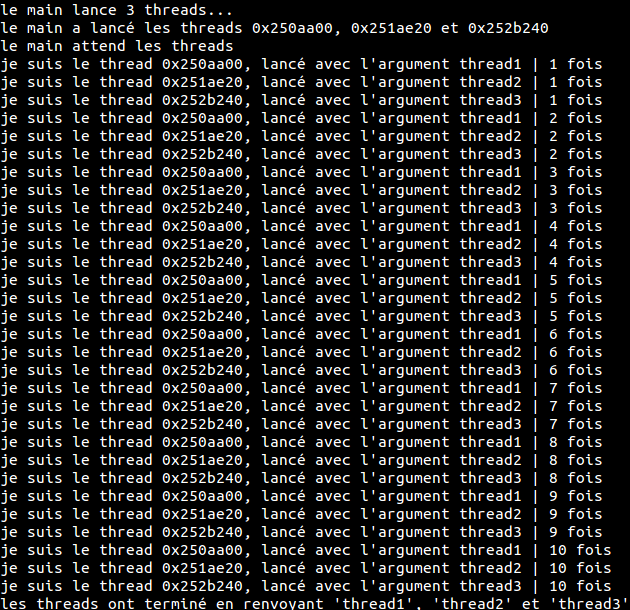
\includegraphics[width=8cm]{fifo.png}
      \caption{Ordonnancement FIFO}
      \label{fifo}
    \end{center}
  \end{minipage}
  \hfill
  \begin{minipage}[c]{.45\linewidth}
    \begin{center}
      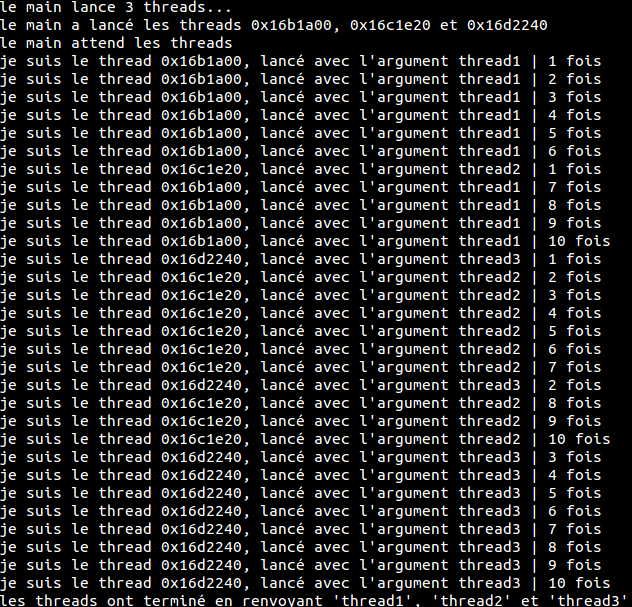
\includegraphics[width=8cm]{prio.png}
      \caption{Ordonnancement priorité}
      \label{prio}
    \end{center}
  \end{minipage}
\end{figure}

